\section{Ejercicio 1}

Peso asignado: 9.

\subsection{Introducción}

Se tiene un mapa de $N$ esquinas y $M$ calles bidireccionales en donde las
esquinas pueden ser casas de alumnos de secundaria, escuelas o esquinas
neutrales. El problema consiste en encontrar la mínima cantidad de esquinas en
las que podemos podemos poner a un estudiante del departamento a contar sobre
la carrera de Ciencias de la Computación, de modo tal que no importe qué
camino utilice cada chico para llegar de su casa al colegio, ni a qué colegio
vaya cada chico, siempre tenga que pasar por una esquina donde lo podamos
interceptar para contarle de la carrera.

\subsection{Solución propuesta}

La resolución de este ejercicio consiste en modelar el mapa como un grafo, y
más específicamente como una red de flujo, y obtener el flujo máximo. En esta
red de flujo se tiene las casas de los estudiantes conectadas a la fuente y
las escuelas al sumidero (pero podría ser al revés y no afectaría en lo
absoluto).

Las capacidades de las aristas serán de 1, pero además también deben tener
capacidad 1 los nodos. Para modelar las capacidades de los vértices, se
representó cada uno de ellos como un arco de capacidad 1 cuyos extremos son un
nodo en donde inciden todas las aristas que incidirían en el vértice original
y otro con todas las aristan salientes.

\begin{figure}[H]
\centering
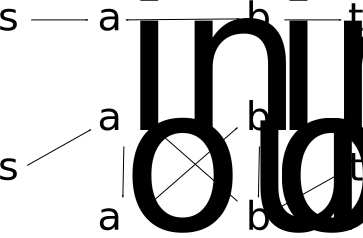
\includegraphics[scale=0.6]{imagenes/ej1_capacidades_nodos.pdf}
\end{figure}

Se construye la red residual y luego se aplica el ya conocido algoritmo de
\textit{Edmonds-Karps} para conocer el flujo máximo.

\subsubsection*{Detalles implementativos}

La estructura utilizada para la representación de la red fue un vector de
listas de enteros (lista de adyacencias). Se reservaron las dos primeras
posiciones del vector para la fuente(0) y el sumidero(1).

El modelado de vértices con capacidades através de aristas con un nodo para
las entradas y otro para las salidas se realiza en el momento mismo de la
lectura de la entrada. El vector de listas contiene exactamente $2N + 2$
elementos, siendo $N$ la cantidad de esquinas. Esto se debe a que por cada
esquina existirán dos nodos(el de entrada y el de salida) y se tiene dos
espacios mas para la fuente y el sumidero.

Al realizar la lectura se tienen dos ciclos. El primero lee el tipo de cada
esquina. Si es una casa de alumno entonces se agrega el nodo de entrada a los
vecinos de la fuente. Si es escuela se agrega el sumidero a los vecinos de el
nodo de salida. Y si es una esquina neutral no se tiene un trato especial.
Para los tres casos se agrega el nodo de salida como único incidido por el
nodo de entrada.

El segundo ciclo simplemente realiza la lectura de ejes, agregando el nodo de
entrada de uno como incidido por el nodo de salida del otro y viceversa.

Una vez hecho esto ya se tiene una red lista para ser procesada.

\subsubsection*{Pseudocódigo}


\begin{algorithm}[]
	\caption{flujoMáximo}
	\Input{$Vector<Lista<Entero>>$ $redResidual$}
	\Output{$Entero$ $flujoMaximo$}

	$flujo$ $\gets$ 0 \;
	$Lista<Entero>$ $camino$ $\gets$ BFS($redResidual$, FUENTE, SUMIDERO) \;
	\While{$\neg camino$.vacio()} {
		recorrerCaminoDeAumento($redResidual$, $camino$) \;
		$camino$ $\gets$ BFS($redResidual$, FUENTE, SUMIDERO) \;
		$flujo$ $\gets$ $flujo + 1$ \;
	}
	\Return $flujo$ \;
\end{algorithm}

\begin{algorithm}[]
	\caption{recorrerCaminoDeAumento}
	\Input{$Vector<Lista<Entero>>$ $redResidual$(por referencia), $Lista<Entero>$ $camino$}

	$Iterador<Lista<Entero>>$ $itCamino$ $\gets$ $camino$.Primero() \;
	\While{$itCamino$.siguiente() $\not=$ $camino$.Fin()} {
		Entero $desde$ $\gets$ *$itCamino$ \;
		Entero $hasta$ $\gets$ *($itCamino$.siguiente()) \;
		$redResidual$[$desde$].borrar($hasta$) \;
		$redResidual$[$hasta$].agregar($desde$) \;
		$itCamino$++ \;
	}
\end{algorithm}

Notar que en recorrerCaminoDeAumento se borran y agregan aristas porque las
capacidades de las mismas son siempre 1. De lo contrario habría que tenerse en
cuenta la capacidad de las mismas, no se borrarían y agregarían sino que se
aumentaría o restaría el flujo que pasa por el eje.

\subsection{Correctitud}

Lo que el algoritmo debe devolver es la minima cantidad de esquinas a donde
puedan situarse estudiantes de modo tal que cada alumno de secundaria siempre
tenga que pasar por una de estas esquinas sin importar que camino tome o a que
colegio vaya.

En otras palabras, existen conjuntos de esquinas para los cuales todos los
caminos de las casas a las escuelas pasan por al menos una de las esquinas del
conjunto. El que interesa es el de mínimo cardinal (un conjunto que tenga
todas las esquinas por supuesto que cumpliría el requisito de interceptar los
alumnos, pero no sería mínimo).

Este conjunto de mínimo cardinal representa un cuello de botella en cuanto a
los caminos que los alumnos de secundaria pueden elegir.

Lo que el algoritmo devuelve es el valor flujo máximo. Por teorema se sabe que
el valor del flujo máximo es igual a la capacidad del corte mínimo.

Lo que hace que la capacidad del corte mínimo en esta red de flujo represente
el cardinal del conjunto de esquinas es el hecho de que los vértices tengan
capacidad 1. Esto provoca que la capacidad del corte no este dada por la
capacidad de las aristas salientes sino por la cantidad de nodos del corte que
tienen aristas salientes. Entonces si para cualquier corte de esta red de
flujo, su capacidad es igual a la cantidad de nodos con aristas salientes, es
decir, esquinas de las cuales salen caminos, consiguiendo el corte mínimo se
obtendría el cuello de botella y su capacidad sería el cardinal del conjunto.

Entonces el valor del flujo máximo de esta red es la mínima cantidad de
esquinas en las que deben situarse estudiantes para poder interceptar a todos
los alumnos sin importar qué caminos tomen o a qué escuela asistan.

\subsection{Complejidad}

Lo primero a analizar es la lectura de la entrada. Previamente se detalló el
procedimiento que constaba de dos ciclos. El primero lee las $N$ esquinas y al
hacerlo las agrega a la correspondiente lista en tiempo constante, por lo que
ese ciclo tiene complejidad temporal $\ord(N)$. El segundo lee las $M$ calles
y también realiza la correspondiente inclusión en una lista en tiempo
constante, por lo que la complejidad es $\ord(M)$. La complejidad temporal de
la lectura es $\ord(M + N)$.

Hecho esto la cantidad de nodos de la red de flujo es de $2N + 2$ debido a que
cada nodo es representado por una arista como fue especificado anteriormente,
lo cual inserta dos nodos por esquina, y a que se tiene dos nodos adicionales
que representan la fuente y el sumidero. La cantidad de aristas es $2M + N$
porque por cada calle se agregan 2 aristas ya que son bidireccionales, y cada
esquina también es una arista.

Si a este grafo se le aplica el algoritmo de \textit{Edmonds-Karps}, que es
$\ord(E^2V)$, la complejidad queda $\ord((2M + N)^2(2N + 2))$.

Como el grafo es conexo ya que existe un camino entre cada par de esquinas se
sabe que $N \leq M + 1$ por lo que podemos acotarlo quedando de esta forma la
complejidad $\ord((2M + M + 1)^2(2N + 2)) = \ord(M^2N)$.

\subsection{Casos de prueba}

Para evaluar el código desarrollado además de ver que diera los resultados
correctos en las entradas provistas por el enunciado se realizaron las
siguientes pruebas:

\begin{itemize}
	\item Camino simple
	\item Grafo moño: este grafo es el que tiene muchas casas, muchas
	escuelas, y todas pasan por una única esquina neutral, siendo esta el
	cuello de botella.
	\item Caminos atravesados: este grafo es el representado en la figura
	\ref{ej1:atravesados}. El propósito de esta prueba es chequear el correcto
	funcionamiento de la red residual y los caminos de aumento. Debido a la
	topología del grafo es posible que el \textit{BFS} devuelva el camino en
	zigzag. Al tocar los nodos que el siguente camino contemplará debe tenerse
	cuidado de no haber manipulado de forma errónea los el camino de aumento
	de manera tal que el segundo camino encontrado no este cortado.
	\item Una casa y una escuela: estos dos casos cumplen el propósito de
	corroborar que las escuelas y casas hayan sido teniadas en cuenta como
	posibles cuellos de botella, no solamente las esquinas neutrales.
	\item Casos normales grandes donde se prueba el algoritmo en general.
\end{itemize}

\begin{figure}[H]
	\caption{Caminos atravesados}
	\label{ej1:atravesados}
	\centering
	\begin{tikzpicture}[x=1.3cm ,y=1.3cm]
		\SetGraphUnit{2}
		\GraphInit[vstyle=Normal]
		\Vertex[L=$A_1$]{A1}
		\EA[L=$A_2$](A1){A2}
		\SO[L=$X_1$](A1){X1}
		\SO[L=$X_2$](A2){X2}
		\SO[L=$X_3$](X1){X3}
		\SO[L=$E_1$](X3){E1}
		\SO[L=$E_2$](X2){E2}
		\Edge(A2)(X2)
		\Edge(X3)(X1)
		\Edge(X3)(E1)
		\SetUpEdge[style={ultra thick}, color=red]
		\Edge(A1)(X1)
		\Edge(X2)(X1)
		\Edge(X2)(E2)
	\end{tikzpicture}
\end{figure}